\clearpage
\subsection{Consideraciones técnicas, operativa y ambientales para la implementación de la mejora}

\subsubsection{Stack tecnológico y arquitectura del sistema}
En esta sección se detallará por completo el stack tecnológico, las medidas de seguridad y la arquitectura que se eligieron para el desarrollo del sistema, 
junto con una breve justificación e implementación de este. 

\subsubsubsection{Tecnologías del Backend}

\textbf{TypeScript.} Se escogió este lenguaje de programación para el backend, cuya principal característica es ser un lenguaje de tipado estático ideal para operaciones clave, 
    donde el tipo de valor no debe variar. \par

\textbf{NestJS.} Framework de Node.js orientado a servidores backend para la construcción progresiva de aplicaciones de mediano a gran escalado empresarial, 
    ofreciendo una estructura base para proyectos, además de su arquitectura modular que permitirá separar responsabilidades de manera efectiva. 
    A diferencia del framework de Express, que no tiene una estructura definida inicialmente. \par

\textbf{Fastify.} Se optó por usar el motor HTTP de Fastify para mejor tiempo y serialización de respuesta JSON, 
    reemplazando el motor de Express que NestJS usaba por defecto. \par

\textbf{PrismaORM.} Librería escogida como puente de comunicación entre la base de datos relacional y el servidor backend para la persistencia y lectura de datos, 
    teniendo gran sinergia con TypeScript; esto asegura la integridad de los datos y protección ante inyecciones SQL. \par

\textbf{Argon2 y AES-256-GCM.} Algoritmos de hash y cifrado utilizados para la protección de contraseñas y datos sensibles, respectivamente. \par

\textbf{JWT y Passport.} Se utilizaron JWT y Passport para el control de sesiones y acceso de las peticiones a la aplicación, 
    permitiendo que la autenticación no dependa de lecturas y solicitudes constantes a la base de datos. \par

\textbf{BullMQ e IORedis.} Herramientas para la gestión de tareas asincrónicas y procesamiento de tareas pesadas en segundo plano, 
    dando una alta disponibilidad a la aplicación y concurrencia a las peticiones de los usuarios para este tipo de tareas. \par

\textbf{WebSocket.} Protocolo de comunicación usado para el envío de notificaciones de tareas hacia los usuarios, 
    mensajes administrativos o eventos cercanos. \par

\textbf{Librerías de Procesamiento y Reportes.} Librerías para la lectura y escritura de documentos empresariales 
    para su posterior procesamiento en procesos de alta demanda en el servidor. \par

\textbf{OpenAPI.} Para la documentación de la API se usaron estas tecnologías para detallar de manera técnica y 
    automática el contrato de los endpoints establecidos en el sistema. \par

\textbf{Jest.} Framework de pruebas para garantizar la funcionalidad de los procesos y la lógica de negocio, 
    realizando pruebas aisladas que permiten minimizar regresiones en el código y asegurar que las funciones garanticen una respuesta predecible y acorde a su desarrollo. \par

\textbf{Dotenv.} Librería de manejo de variables de entorno para garantizar la seguridad de llaves de servicios, 
    firmas de encriptado y contraseñas de base de datos.\par

\subsubsubsection{Tecnologías del Frontend}
\textbf{React 19.} Librería de JavaScript/TypeScript utilizada para la creación de componentes reutilizables y gestionar el renderizado de estos de manera eficiente.\par
\textbf{TypeScript 6.} Lenguaje de tipado estático que permite la integridad y asegurar el tipo de valores de los datos, para su posterior envío al backend.\par
\textbf{Vite 8.} Empaquetador, servidor de desarrollo rápido para la compilación de la aplicación.\par
\textbf{Tailwind CSS.} Framework basado en CSS, que permite diseñar interfaces modernas sin salir del código HTML/TSX.\par
\textbf{Shadcn/ui.} Colección de componentes reutilizables ya creados anteriormente, altamente personalizable (botones, tablas, entre otros).\par
\textbf{lucide-react.} Librería de iconos vectoriales ligeros, que permite dar orientación al usuario dentro de la aplicación.\par
\textbf{TanStack Query 5.} Sincronización de caché, carga y actualización de datos que vienen por parte del servidor.\par
\textbf{Zustand 5.} Librería de gestión de estado global, que permite guardar sesión y compartir datos entre pantallas.\par
\textbf{Axios.} Cliente HTTP para realizar solicitudes al backend y obtener respuestas de manera eficiente.\par
\textbf{React Hook Form 7.} Librería para el manejo de formularios, reduciendo cargas innecesarias al escribir.\par
\textbf{Zod.} Librería de validación de datos, permite la comparación y estructura del envío de datos al backend.\par
\textbf{React Router DOM 7.} Sistema de navegación para gestionar distintas páginas de la aplicación web sin recargar la página completa.\par
\subsubsubsection{Paquete de validación de Schemas compartido.} 
Paquete independiente que permite centralizar la validación de schemas, tipos de datos y reglas de estas. \par

\textbf{ZOD.} Librería para validación de datos, perfecta para establecer contratos de entrada a los endpoints de la aplicación.

\subsubsubsection{Bases de Datos}
Se escogió usar una base de datos para permanencia de registros historicos, centralizacion, lectura y auditoria de estos.

\textbf{PostgreSQL.} Motor de base de datos relacional elegido por su robustez, 
    ideal para proyectos empresariales garantizando la estructura de guardado de los datos de los usuarios. \par

\textbf{Redis.} Sistema de almacenamiento de datos en memoria, 
    de alto rendimiento en procedimientos de caché y colas, para la concurrencia en el servidor. \par

\textbf{UUIDv7.} Método de identificación a entidades dentro de la base de datos relacional; 
    a diferencia de sus versiones anteriores que generan el identificador de manera aleatoria, 
    este realiza la generación mediante orden cronológico, lo cual ayuda a auditar la creación de registros. \par

\subsubsubsection{Criptografía y Seguridad de Datos}
En esta sección se explicarán los mecanismos internos para garantizar la integridad de los datos del usuario al momento de hacer persistencia 
y peticiones dentro y fuera de la base de datos.

\textbf{Enmascaramiento de datos.} Técnica para la protección de datos de los usuarios en las respuestas JSON de los endpoints, 
    que consiste en que una parte del valor que almacena la variable sea reemplazada por otro carácter. \par

\textbf{Cifrado de datos.} Técnica para la protección de datos, consiste en transformar un dato legible a uno ilegible antes de ser enviado 
    a la base de datos para garantizar que, en caso de una fuga de información, los datos no sean capaces de ser leídos por el atacante.

\subsubsubsection{Diagrama de Arquitectura de Software}

La solución tecnológica adopta un patrón arquitectónico de \textbf{Monolito Modular orientado a Casos de Uso} (\textit{Use-Case Driven Modular Monolith}), 
estructurado bajo los principios de separación de responsabilidades y modularidad transversal. 
Esta disposición técnica organiza la lógica del negocio en dominios delimitados sin incurrir en sobreingeniería de interfaces abstractas, 
garantizando un mantenimiento ágil, escalabilidad vertical y una estricta coherencia transaccional (Figura~\ref{fig:arquitectura_backend}):

\begin{enumerate}[leftmargin=*]
    
    \item \textbf{Capa de Presentación y Acceso (Cliente Web SPA):} Implementada como una aplicación de página única mediante React~19, TypeScript y empaquetada con Vite. 
    La interfaz de usuario se compone mediante componentes atómicos y accesibles provistos por Shadcn y estilizados con Tailwind CSS. 
    La sincronización y gestión de la caché del servidor en el navegador recae sobre TanStack Query v5, 
    mientras que el estado de sesión y navegación se administra de forma reactiva con Zustand. 
    La comunicación hacia el servidor se efectúa mediante solicitudes HTTP asíncronas bajo el estándar REST con cabeceras de autorización Bearer (tokens JWT en cookies HttpOnly seguras), 
    complementándose con un canal bidireccional mediante WebSockets/SSE para la emisión de alertas operativas en tiempo real (notificaciones de aprobación de tareas, vencimientos de contratos e incidencias).
    
    \item \textbf{Capa de Aplicación y Núcleo Transaccional (NestJS Engine):} Utiliza como motor perimetral el adaptador de alto rendimiento \textbf{Fastify~5}, 
    optimizado para maximizar el \textit{throughput} de peticiones y acelerar la serialización JSON. 
    El procesamiento HTTP atraviesa un pipeline perimetral estructurado:
    
    \begin{itemize}
        \item \textit{Guards de Autenticación y Autorización (RBAC):} Verifican la integridad criptográfica del token JWT y 
        contrastan los permisos del actor contra la matriz de roles corporativos definida en el sistema (Administrador, RRHH, Contador, Asistente y Colaborador/Empleado).
        
        \item \textit{Pipes de Validación Just-In-Time (JIT):} Sancionan y sanitizan la estructura de las cargas entrantes
         contra la fuente única de verdad compartida (\texttt{@jyp/shared-contracts}), 
         validando esquemas fuertemente tipados mediante \textbf{Zod} antes de comprometer memoria en la capa de negocio. 
         Las respuestas erróneas se estandarizan bajo la norma \textbf{RFC~7807} (\textit{Problem Details for HTTP APIs}).
        
        \item \textit{Segmentación en Módulos de Dominio y Casos de Uso:} La lógica de negocio abandona los servicios monolíticos extensos 
        y se estructura en submódulos encapsulados regidos por comandos atómicos (\textit{Use Cases}):
        
        \begin{itemize}
            \item \textbf{Módulo Core:} Centraliza la autenticación (hashing con Argon2id), el ciclo de vida de usuarios, perfiles y la bitácora inmutable de auditoría.
            \item \textbf{Módulo RR.HH.:} Administra la estructura organizacional (áreas, cargos, empleados y jornadas), 
                                           el ciclo contractual con alertas de vencimiento, derechohabientes, datos financieros de los empleados, trámites documentarios 
                                           y la ingesta masiva de legajos con adaptador tolerante a fallos hacia la API de RENIEC.
            \item \textbf{Módulo Asistencia:} Procesa la lectura y normalización de marcaciones biométricas (ingesta por streaming), 
                                               la evaluación diaria de ausencias y tardanzas, el cálculo de jornadas laborales y la gestión de incidencias con firmas hash SHA-256.
            \item \textbf{Módulo Nóminas:} Gobierna los parámetros legales (UIT, RMV, horas extras), la matriz previsional de AFPs/ONP
                                                     y el cálculo mensual y extraordinario (Gratificaciones, CTS, Liquidaciones), asegurando el congelamiento contable inmutable del periodo.
            \item \textbf{Módulo Integraciones:} Implementa el patrón \textit{Transactional Outbox} para estructurar solicitudes de exportación legal y habilitar un canal seguro máquina a máquina (M2M) 
                                                  autenticado mediante firmas HMAC-SHA256.
        \end{itemize}
        
        \item \textit{Seguridad y Persistencia Transaccional:} Los datos financieros altamente sensibles 
            (cuentas sueldo y códigos interbancarios CCI) son encriptados simétricamente en reposo mediante el algoritmo \textbf{AES-256-GCM} con enmascaramiento dinámico en lecturas. 
            A nivel de infraestructura, Prisma ORM gestiona transacciones atómicas interactivas (\texttt{\$transaction}) 
            vinculando el contexto del usuario ejecutor a disparadores (\textit{triggers}) nativos de auditoría en la base de datos.
    \end{itemize}

    \item \textbf{Capa de Procesamiento Asíncrono y Orquestación (BullMQ y n8n):} 
        Para prevenir el bloqueo del bucle de eventos (\textit{Event Loop}) de Node.js durante operaciones intensivas de CPU e I/O, el sistema delega la carga computacional pesada:
    \begin{itemize}
        \item \textit{Colas en Memoria con Redis 7 y Pool de Workers:} El cálculo masivo de planillas y la validación de archivos voluminosos se despachan a colas gestionadas por BullMQ y Redis. 
                                                                        Un grupo de hilos nativos secundarios (\textit{Worker Threads} vía Piscina) procesa los algoritmos financieros en aislamiento de memoria, 
                                                                        utilizando aritmética decimal exacta (\texttt{decimal.js}) y optimizaciones de consultas agrupadas (\textit{Bulk Fetch}) 
                                                                        para erradicar el problema $N+1$.
        
        \item \textit{Orquestador de Automatizaciones n8n:} Desplegado en un contenedor independiente, actúa como ejecutor asíncrono secundario. 
                                                             Tras la aprobación y congelamiento de la nómina, 
                                                             n8n recibe un webhook disparador verificado con HMAC-SHA256 para compilar las estructuras posicionales oficiales 
                                                             (archivos \texttt{.rem} y \texttt{.jor} de la PLAME SUNAT, formato de 141 posiciones de AFPnet y transferencias masivas de Telecrédito BCP), 
                                                             renderizar las boletas de pago en PDF protegidas con el DNI del trabajador y distribuirlas masivamente vía SMTP.
    \end{itemize}

    \item \textbf{Capa de Persistencia e Infraestructura Relacional:} Descansa sobre un motor de base de datos relacional \textbf{PostgreSQL~16}, 
                                                                        utilizando identificadores ordenados cronológicamente (\textbf{UUIDv7}) para garantizar inserciones secuenciales desfragmentadas en los índices B-Tree, 
                                                                        y disparadores PL/pgSQL que imponen inmutabilidad física sobre las tablas de planillas congeladas y registros de auditoría.
\end{enumerate}

\par\medskip
\noindent
\begin{minipage}{\linewidth}
    \linespread{1}\footnotesize
    \refstepcounter{figure}\label{fig:arquitectura_backend}
    \addcontentsline{lof}{figure}{Figura~\thefigure. Diagrama de arquitectura general del sistema web de nóminas}
    {\bfseries Figura~\thefigure}\par
    {\itshape Diagrama de arquitectura general del sistema web de nóminas}\par
    \vspace{4pt}
    \makebox[\linewidth][c]{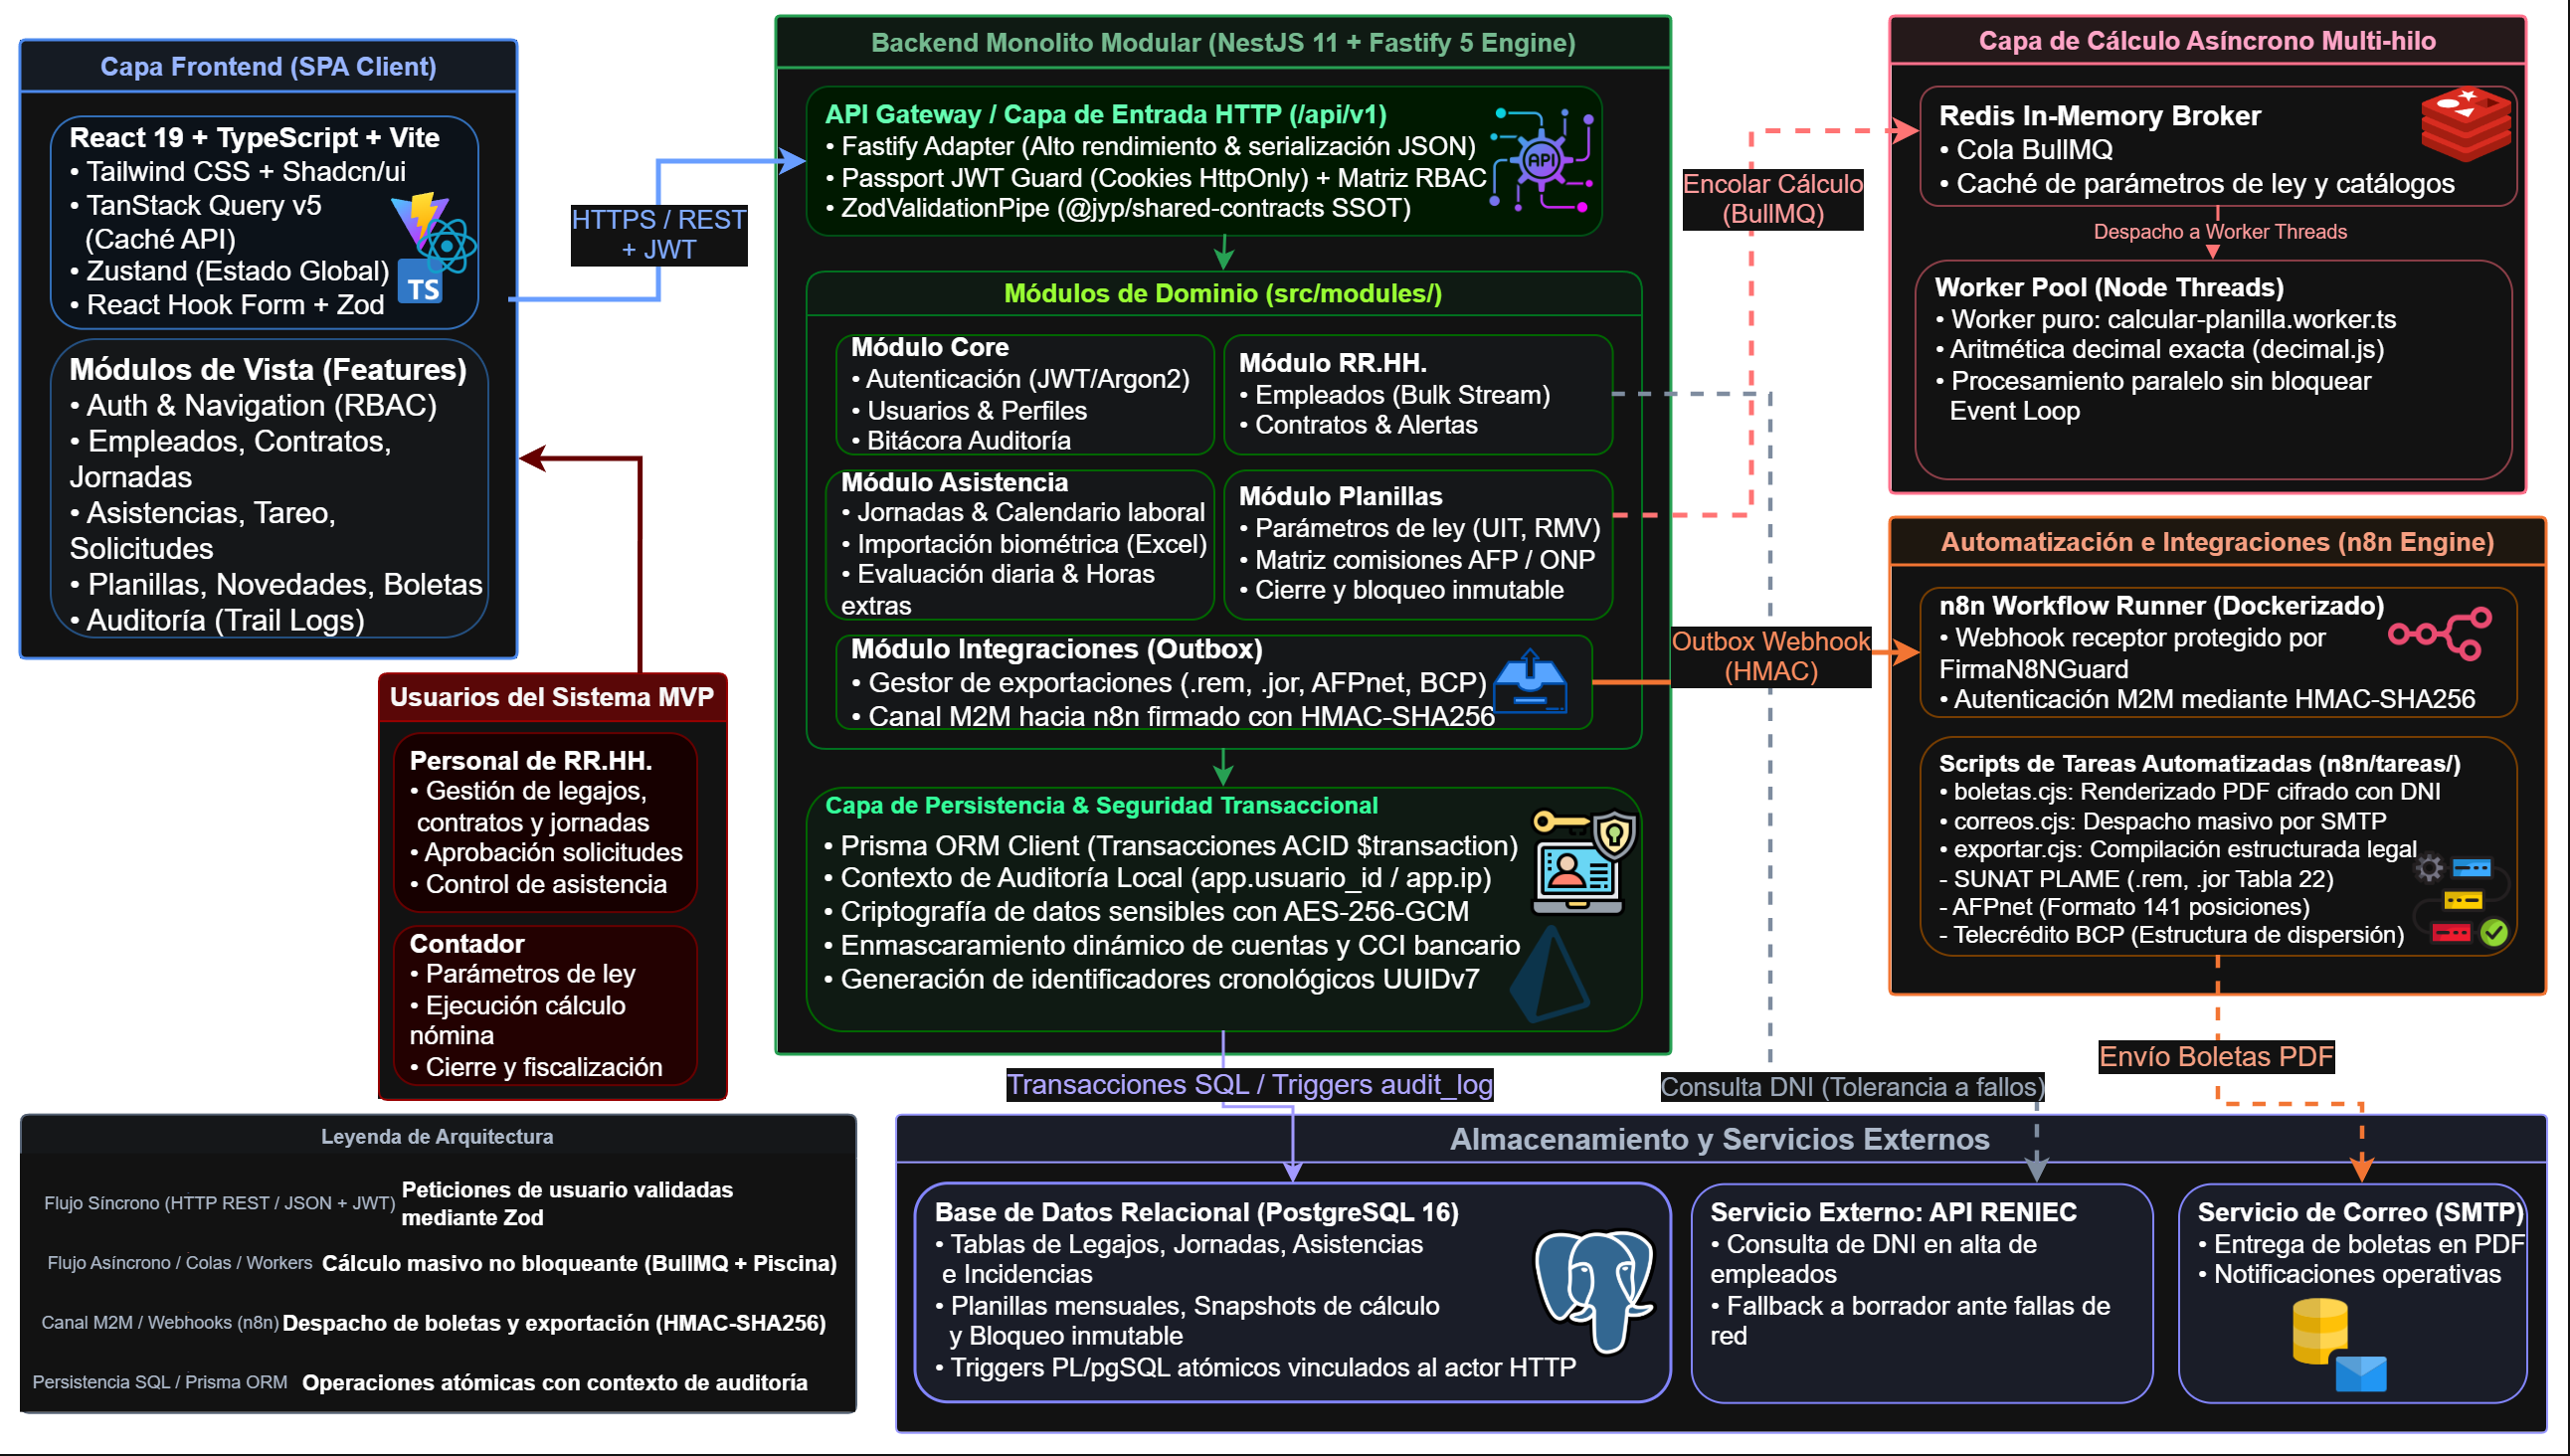
\includegraphics[
        width=\linewidth,
        height=0.76\textheight,
        keepaspectratio
    ]{images/diagramaFuncionamientoGeneral.png}}\par
    \vspace{4pt}
    \textit{Nota.} Estructura modular en capas, procesamiento asíncrono y automatización con n8n. Elaboración propia; los logotipos, 
    marcas e isotipos integrados son propiedad de sus respectivos titulares y se utilizan únicamente con fines ilustrativos y académicos.\par
\end{minipage}
\finBloqueAPA
